% Options for packages loaded elsewhere
\PassOptionsToPackage{unicode}{hyperref}
\PassOptionsToPackage{hyphens}{url}
%
\documentclass[
  ignorenonframetext,
]{beamer}
\usepackage{pgfpages}
\setbeamertemplate{caption}[numbered]
\setbeamertemplate{caption label separator}{: }
\setbeamercolor{caption name}{fg=normal text.fg}
\beamertemplatenavigationsymbolsempty
% Prevent slide breaks in the middle of a paragraph
\widowpenalties 1 10000
\raggedbottom
\setbeamertemplate{part page}{
  \centering
  \begin{beamercolorbox}[sep=16pt,center]{part title}
    \usebeamerfont{part title}\insertpart\par
  \end{beamercolorbox}
}
\setbeamertemplate{section page}{
  \centering
  \begin{beamercolorbox}[sep=12pt,center]{part title}
    \usebeamerfont{section title}\insertsection\par
  \end{beamercolorbox}
}
\setbeamertemplate{subsection page}{
  \centering
  \begin{beamercolorbox}[sep=8pt,center]{part title}
    \usebeamerfont{subsection title}\insertsubsection\par
  \end{beamercolorbox}
}
\AtBeginPart{
  \frame{\partpage}
}
\AtBeginSection{
  \ifbibliography
  \else
    \frame{\sectionpage}
  \fi
}
\AtBeginSubsection{
  \frame{\subsectionpage}
}
\usepackage{amsmath,amssymb}
\usepackage{lmodern}
\usepackage{iftex}
\ifPDFTeX
  \usepackage[T1]{fontenc}
  \usepackage[utf8]{inputenc}
  \usepackage{textcomp} % provide euro and other symbols
\else % if luatex or xetex
  \usepackage{unicode-math}
  \defaultfontfeatures{Scale=MatchLowercase}
  \defaultfontfeatures[\rmfamily]{Ligatures=TeX,Scale=1}
\fi
\usetheme[]{Ilmenau}
% Use upquote if available, for straight quotes in verbatim environments
\IfFileExists{upquote.sty}{\usepackage{upquote}}{}
\IfFileExists{microtype.sty}{% use microtype if available
  \usepackage[]{microtype}
  \UseMicrotypeSet[protrusion]{basicmath} % disable protrusion for tt fonts
}{}
\makeatletter
\@ifundefined{KOMAClassName}{% if non-KOMA class
  \IfFileExists{parskip.sty}{%
    \usepackage{parskip}
  }{% else
    \setlength{\parindent}{0pt}
    \setlength{\parskip}{6pt plus 2pt minus 1pt}}
}{% if KOMA class
  \KOMAoptions{parskip=half}}
\makeatother
\usepackage{xcolor}
\newif\ifbibliography
\usepackage{color}
\usepackage{fancyvrb}
\newcommand{\VerbBar}{|}
\newcommand{\VERB}{\Verb[commandchars=\\\{\}]}
\DefineVerbatimEnvironment{Highlighting}{Verbatim}{commandchars=\\\{\}}
% Add ',fontsize=\small' for more characters per line
\usepackage{framed}
\definecolor{shadecolor}{RGB}{248,248,248}
\newenvironment{Shaded}{\begin{snugshade}}{\end{snugshade}}
\newcommand{\AlertTok}[1]{\textcolor[rgb]{0.94,0.16,0.16}{#1}}
\newcommand{\AnnotationTok}[1]{\textcolor[rgb]{0.56,0.35,0.01}{\textbf{\textit{#1}}}}
\newcommand{\AttributeTok}[1]{\textcolor[rgb]{0.77,0.63,0.00}{#1}}
\newcommand{\BaseNTok}[1]{\textcolor[rgb]{0.00,0.00,0.81}{#1}}
\newcommand{\BuiltInTok}[1]{#1}
\newcommand{\CharTok}[1]{\textcolor[rgb]{0.31,0.60,0.02}{#1}}
\newcommand{\CommentTok}[1]{\textcolor[rgb]{0.56,0.35,0.01}{\textit{#1}}}
\newcommand{\CommentVarTok}[1]{\textcolor[rgb]{0.56,0.35,0.01}{\textbf{\textit{#1}}}}
\newcommand{\ConstantTok}[1]{\textcolor[rgb]{0.00,0.00,0.00}{#1}}
\newcommand{\ControlFlowTok}[1]{\textcolor[rgb]{0.13,0.29,0.53}{\textbf{#1}}}
\newcommand{\DataTypeTok}[1]{\textcolor[rgb]{0.13,0.29,0.53}{#1}}
\newcommand{\DecValTok}[1]{\textcolor[rgb]{0.00,0.00,0.81}{#1}}
\newcommand{\DocumentationTok}[1]{\textcolor[rgb]{0.56,0.35,0.01}{\textbf{\textit{#1}}}}
\newcommand{\ErrorTok}[1]{\textcolor[rgb]{0.64,0.00,0.00}{\textbf{#1}}}
\newcommand{\ExtensionTok}[1]{#1}
\newcommand{\FloatTok}[1]{\textcolor[rgb]{0.00,0.00,0.81}{#1}}
\newcommand{\FunctionTok}[1]{\textcolor[rgb]{0.00,0.00,0.00}{#1}}
\newcommand{\ImportTok}[1]{#1}
\newcommand{\InformationTok}[1]{\textcolor[rgb]{0.56,0.35,0.01}{\textbf{\textit{#1}}}}
\newcommand{\KeywordTok}[1]{\textcolor[rgb]{0.13,0.29,0.53}{\textbf{#1}}}
\newcommand{\NormalTok}[1]{#1}
\newcommand{\OperatorTok}[1]{\textcolor[rgb]{0.81,0.36,0.00}{\textbf{#1}}}
\newcommand{\OtherTok}[1]{\textcolor[rgb]{0.56,0.35,0.01}{#1}}
\newcommand{\PreprocessorTok}[1]{\textcolor[rgb]{0.56,0.35,0.01}{\textit{#1}}}
\newcommand{\RegionMarkerTok}[1]{#1}
\newcommand{\SpecialCharTok}[1]{\textcolor[rgb]{0.00,0.00,0.00}{#1}}
\newcommand{\SpecialStringTok}[1]{\textcolor[rgb]{0.31,0.60,0.02}{#1}}
\newcommand{\StringTok}[1]{\textcolor[rgb]{0.31,0.60,0.02}{#1}}
\newcommand{\VariableTok}[1]{\textcolor[rgb]{0.00,0.00,0.00}{#1}}
\newcommand{\VerbatimStringTok}[1]{\textcolor[rgb]{0.31,0.60,0.02}{#1}}
\newcommand{\WarningTok}[1]{\textcolor[rgb]{0.56,0.35,0.01}{\textbf{\textit{#1}}}}
\setlength{\emergencystretch}{3em} % prevent overfull lines
\providecommand{\tightlist}{%
  \setlength{\itemsep}{0pt}\setlength{\parskip}{0pt}}
\setcounter{secnumdepth}{-\maxdimen} % remove section numbering
\setbeamertemplate{navigation symbols}{}
\setbeamertemplate{footline}[page number]
\ifLuaTeX
  \usepackage{selnolig}  % disable illegal ligatures
\fi
\IfFileExists{bookmark.sty}{\usepackage{bookmark}}{\usepackage{hyperref}}
\IfFileExists{xurl.sty}{\usepackage{xurl}}{} % add URL line breaks if available
\urlstyle{same} % disable monospaced font for URLs
\hypersetup{
  pdftitle={Multivariate Analysis},
  hidelinks,
  pdfcreator={LaTeX via pandoc}}

\title{Multivariate Analysis}
\author{Zhaoxia Yu\\
Professor, Department of Statistics}
\date{2023-04-06}

\begin{document}
\frame{\titlepage}

\hypertarget{intro}{%
\section{Intro}\label{intro}}

\hypertarget{introduction}{%
\subsection{Introduction}\label{introduction}}

\begin{frame}{Course Information}
\protect\hypertarget{course-information}{}
\begin{itemize}
\tightlist
\item
  Please use the Canvas website for course materials, important updates,
  and deadlines.
\item
  Announcements will be sent to the mailing list or posted in Canvas.
\item
  Assignment submission: GradeScope on Canvas.
\end{itemize}
\end{frame}

\begin{frame}{Multivriate Data}
\protect\hypertarget{multivriate-data}{}
\begin{itemize}
\tightlist
\item
  ``multi'' means more than one
\item
  Multivariate data: the data with \textcolor{red}{simultaneous
  measurements} on many variables
\end{itemize}

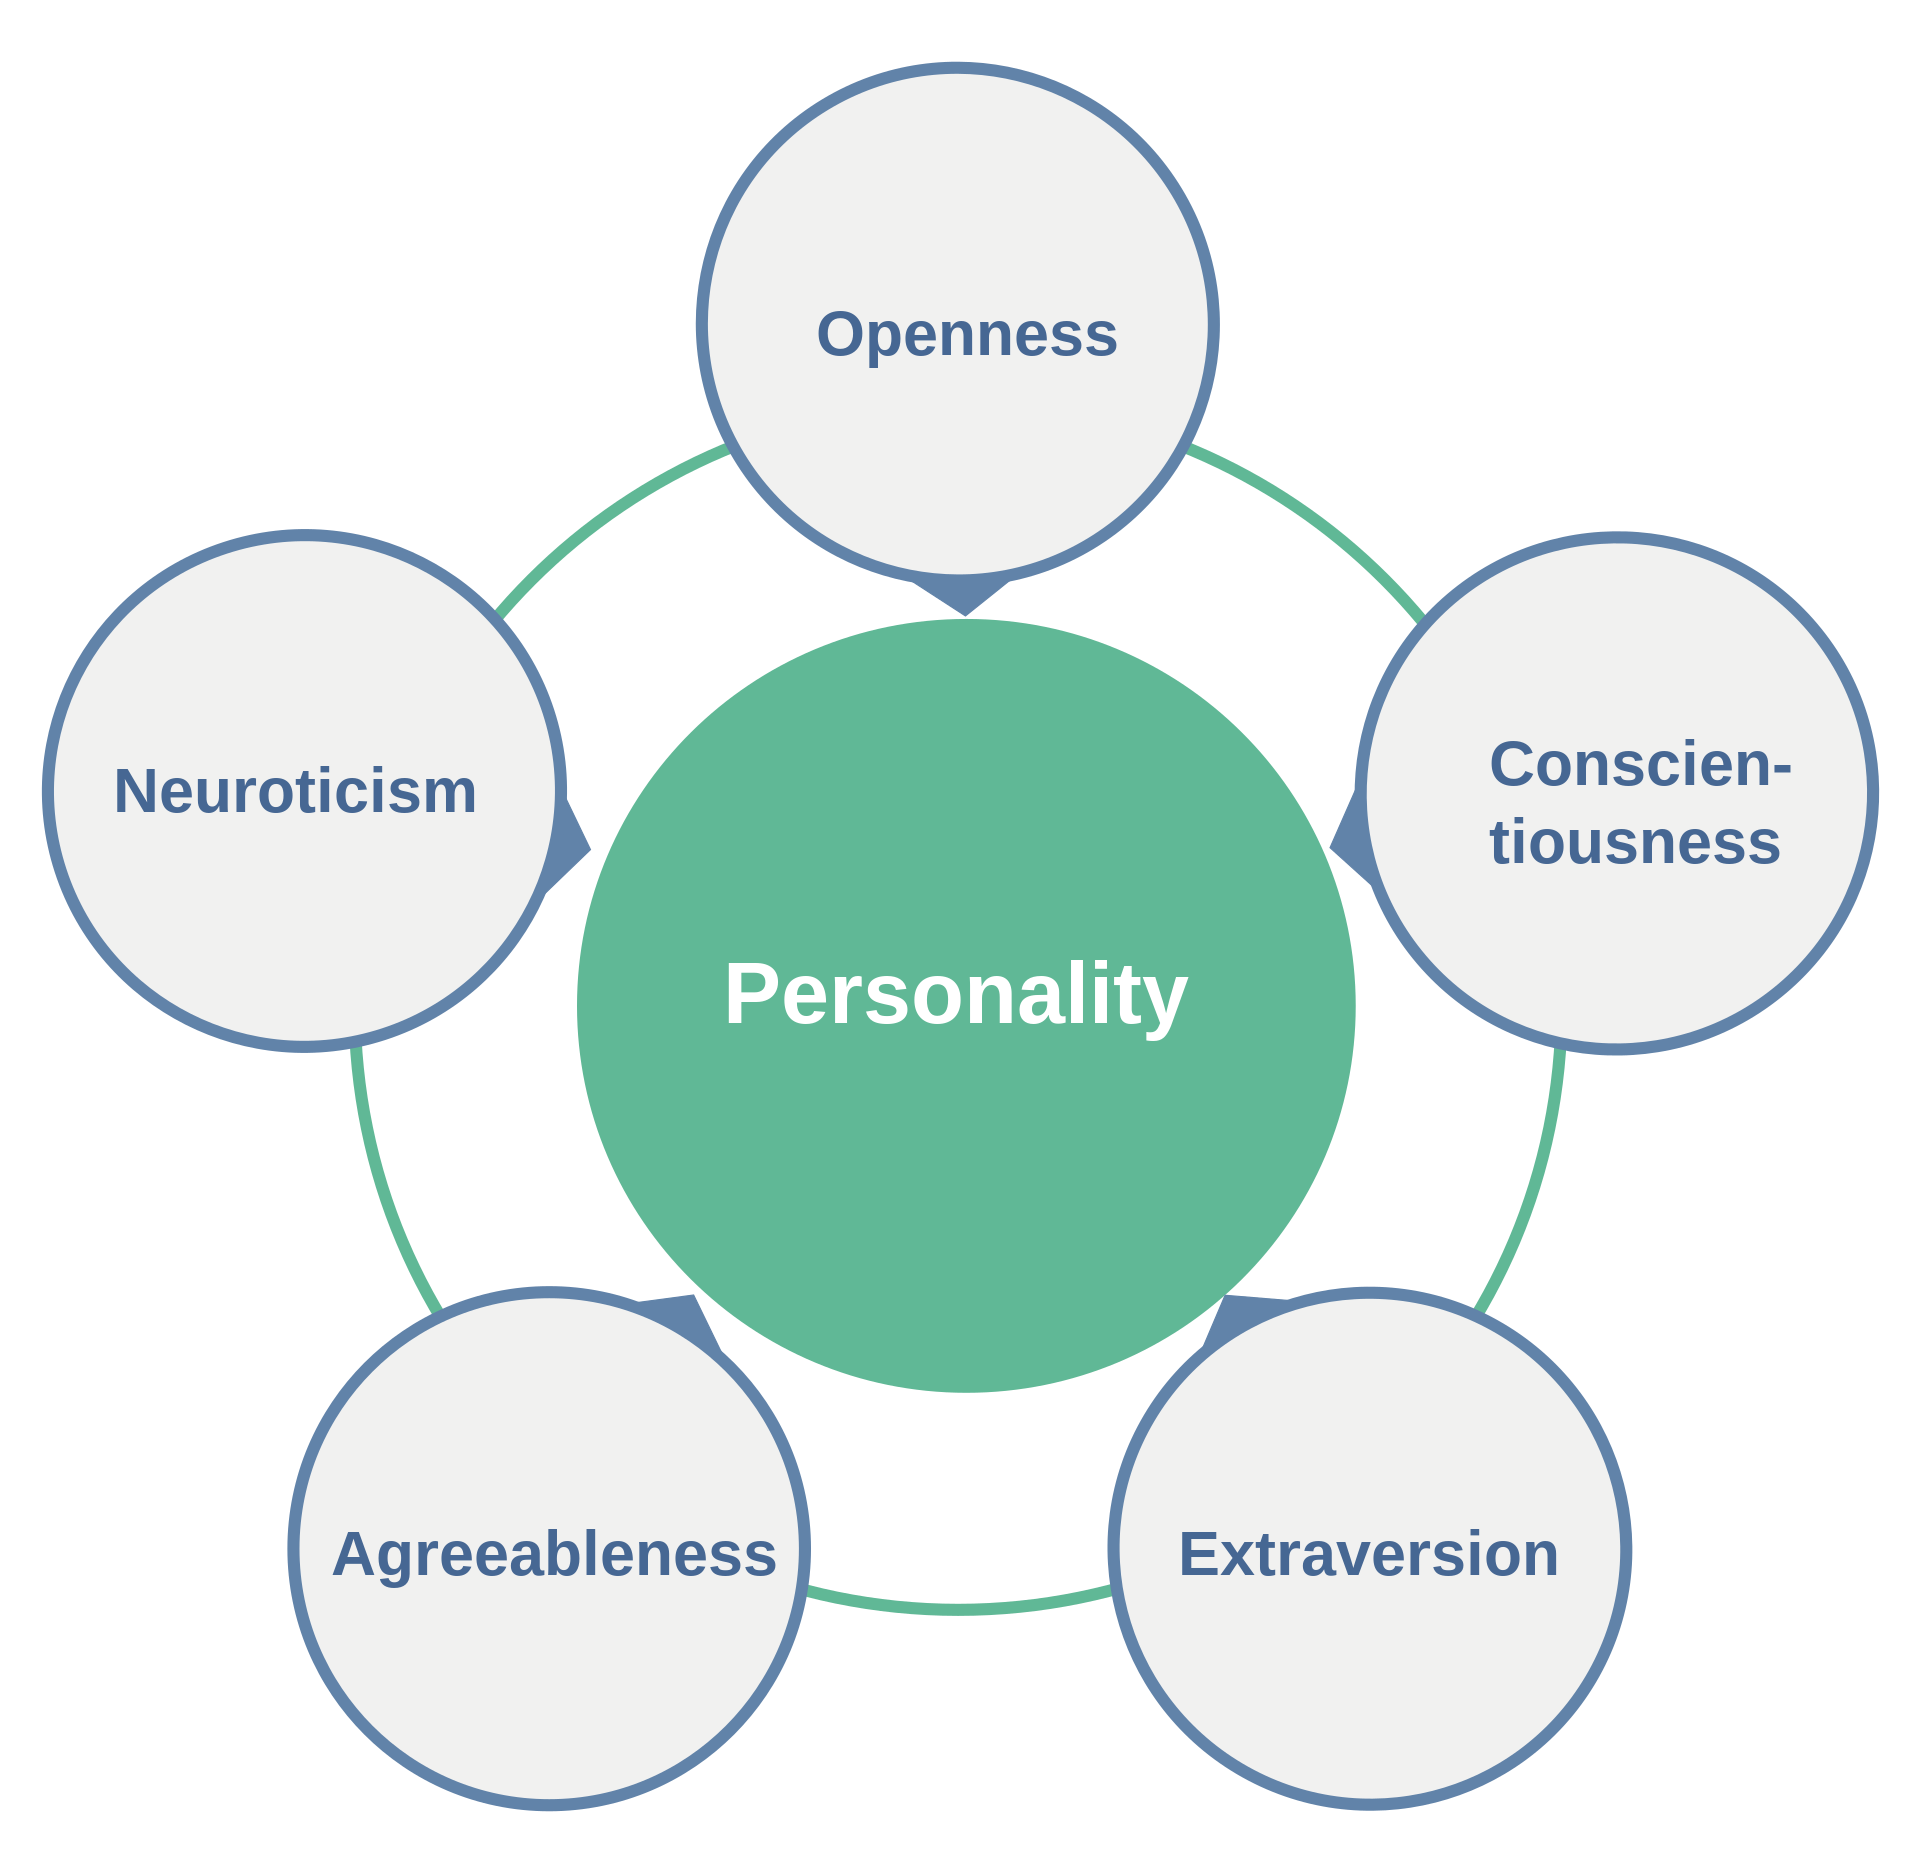
\includegraphics[width=0.5\linewidth]{img/personality}
\end{frame}

\begin{frame}{More Examples of Multivariate Data}
\protect\hypertarget{more-examples-of-multivariate-data}{}
\begin{itemize}
\tightlist
\item
  A basketball player: points, rebounds, steals, assists, turnovers,
  free throws, fouls, etc
\item
  A person's well-being: social, economic, psychological, medical,
  physical, etc
\item
  A person's annual physical exam report
\end{itemize}
\end{frame}

\begin{frame}{What is Multivariate Analysis}
\protect\hypertarget{what-is-multivariate-analysis}{}
\begin{itemize}
\tightlist
\item
  The term ``multivariate analysis'' implies a broader scope than
  univariate analysis.
\item
  Certain approaches like simple linear regression and multiple
  regression are typically not considered as multivariate analysis as
  they tend to focus on the conditional distribution of one univariate
  variable rather than multiple variables.
\item
  Multivariate analysis focuses on the joint behavior of several
  variables simultaneously to identify patterns and relationships
\end{itemize}
\end{frame}

\begin{frame}{Learning Objectives}
\protect\hypertarget{learning-objectives}{}
\begin{itemize}
\tightlist
\item
  Matrix algebra, distributions
\item
  Visualization
\item
  Inference about a mean vector or multiple mean vectors
\item
  Multivariate analysis of variance (MANOVA) and multivariate regression
\item
  Linear discriminant analysis (LDA)
\item
  Principal component analysis (PCA)
\item
  Cluster analysis
\item
  Factor analysis
\end{itemize}
\end{frame}

\begin{frame}{Milestones in the history of multivariate analysis}
\protect\hypertarget{milestones-in-the-history-of-multivariate-analysis}{}
\begin{itemize}
\tightlist
\item
  1901: PCA was invented by Karl Pearson; independently developed by
  Harold Hotelling in the 1930s.
\item
  1904: Charles Spearman introduced factor analysis to identify
  underlying factors that explain the correlation between multiple
  variables.
\item
  1928: Wishart presented the distribution of the covariance matrix of a
  random sample from a multivariate normal distribution.
\item
  1936: Ronald Fisher developed discriminant analysis.
\item
  ????: Cluster analysis.
\item
  1936: Canonical analysis by Harold Hotelling.
\item
  1960s: Multidimensional scaling.
\item
  1970s: Multivariate regression.
\item
  1980s: Structural equation modeling; the idea dated back to
  (1920-1921) by Sewall Wright.
\end{itemize}
\end{frame}

\hypertarget{matrix-algebra}{%
\section{Matrix Algebra}\label{matrix-algebra}}

\hypertarget{vectors-we-begin-with-a-little-bit-matrix-algebra}{%
\subsection{Vectors: We begin with a little bit matrix
algebra}\label{vectors-we-begin-with-a-little-bit-matrix-algebra}}

\begin{frame}[fragile]{Vectors in R}
\protect\hypertarget{vectors-in-r}{}
\begin{itemize}
\tightlist
\item
  There are many ways to create or define a vector
\end{itemize}

\begin{Shaded}
\begin{Highlighting}[]
\NormalTok{x}\OtherTok{=}\FunctionTok{rep}\NormalTok{(}\FloatTok{0.3}\NormalTok{, }\DecValTok{4}\NormalTok{)}
\NormalTok{x}
\end{Highlighting}
\end{Shaded}

\begin{verbatim}
## [1] 0.3 0.3 0.3 0.3
\end{verbatim}

\begin{Shaded}
\begin{Highlighting}[]
\NormalTok{x}\OtherTok{=}\FunctionTok{seq}\NormalTok{(}\DecValTok{1}\NormalTok{, }\DecValTok{4}\NormalTok{, }\AttributeTok{by=}\FloatTok{0.2}\NormalTok{)}
\NormalTok{x}
\end{Highlighting}
\end{Shaded}

\begin{verbatim}
##  [1] 1.0 1.2 1.4 1.6 1.8 2.0 2.2 2.4 2.6 2.8 3.0 3.2 3.4 3.6 3.8 4.0
\end{verbatim}

\begin{Shaded}
\begin{Highlighting}[]
\FunctionTok{c}\NormalTok{(}\StringTok{"a1"}\NormalTok{, }\StringTok{"a2"}\NormalTok{, }\StringTok{"a3"}\NormalTok{)}
\end{Highlighting}
\end{Shaded}

\begin{verbatim}
## [1] "a1" "a2" "a3"
\end{verbatim}
\end{frame}

\begin{frame}[fragile]{Vectors in R}
\protect\hypertarget{vectors-in-r-1}{}
\begin{Shaded}
\begin{Highlighting}[]
\NormalTok{x}\OtherTok{=}\FunctionTok{c}\NormalTok{(}\FloatTok{0.4}\NormalTok{, }\FloatTok{0.2}\NormalTok{, }\FloatTok{0.5}\NormalTok{)}
\NormalTok{x}
\end{Highlighting}
\end{Shaded}

\begin{verbatim}
## [1] 0.4 0.2 0.5
\end{verbatim}

\begin{Shaded}
\begin{Highlighting}[]
\FunctionTok{length}\NormalTok{(x)}
\end{Highlighting}
\end{Shaded}

\begin{verbatim}
## [1] 3
\end{verbatim}

\begin{Shaded}
\begin{Highlighting}[]
\FunctionTok{dim}\NormalTok{(x) }\CommentTok{\#note that there is no dimension information}
\end{Highlighting}
\end{Shaded}

\begin{verbatim}
## NULL
\end{verbatim}
\end{frame}

\begin{frame}[fragile]{A row or column of a matrix is also a vector}
\protect\hypertarget{a-row-or-column-of-a-matrix-is-also-a-vector}{}
\begin{Shaded}
\begin{Highlighting}[]
\NormalTok{x}\OtherTok{=}\FunctionTok{rbind}\NormalTok{(}\FunctionTok{c}\NormalTok{(}\FloatTok{0.4}\NormalTok{,}\FloatTok{0.2}\NormalTok{,}\FloatTok{0.5}\NormalTok{), }\FunctionTok{rep}\NormalTok{(}\DecValTok{1}\NormalTok{,}\DecValTok{3}\NormalTok{))}
\FunctionTok{dim}\NormalTok{(x)}
\end{Highlighting}
\end{Shaded}

\begin{verbatim}
## [1] 2 3
\end{verbatim}

\begin{Shaded}
\begin{Highlighting}[]
\NormalTok{x[}\DecValTok{1}\NormalTok{,]}
\end{Highlighting}
\end{Shaded}

\begin{verbatim}
## [1] 0.4 0.2 0.5
\end{verbatim}

\begin{Shaded}
\begin{Highlighting}[]
\NormalTok{x[,}\DecValTok{1}\NormalTok{]}
\end{Highlighting}
\end{Shaded}

\begin{verbatim}
## [1] 0.4 1.0
\end{verbatim}
\end{frame}

\hypertarget{special-matrices}{%
\subsection{Special Matrices}\label{special-matrices}}

\begin{frame}{Row or Column Vectors}
\protect\hypertarget{row-or-column-vectors}{}
\begin{itemize}
\tightlist
\item
  A vector (column vector) is a special matrix consisting of a single
  column of elements. e.g.,
  \[a=\begin{pmatrix}a_1\\ a_2 \\ a_3\end{pmatrix}\]
\item
  A row vector is a special matrix consisting of a single row of
  elements \[b=(b_1, b_2, b_3, b_4)\]
\item
  In this class, a vector means a column vector
\item
  A row or column vector is also a matrix
\item
  The transpose of a row vector is a column vector; the transpose of a
  column vector is row vector. e.g., \[a'=(a_1,a_2,a_3)\]
\end{itemize}
\end{frame}

\begin{frame}[fragile]{Row or Column Vectors}
\protect\hypertarget{row-or-column-vectors-1}{}
\begin{itemize}
\tightlist
\item
  In vector/matrix operations, it is helpful to define row or column
  vectors
\item
  A row vector
\end{itemize}

\begin{Shaded}
\begin{Highlighting}[]
\FunctionTok{matrix}\NormalTok{(}\FunctionTok{rep}\NormalTok{(}\FloatTok{0.5}\NormalTok{,}\DecValTok{3}\NormalTok{), }\DecValTok{1}\NormalTok{, }\DecValTok{3}\NormalTok{)}
\end{Highlighting}
\end{Shaded}

\begin{verbatim}
##      [,1] [,2] [,3]
## [1,]  0.5  0.5  0.5
\end{verbatim}

\begin{Shaded}
\begin{Highlighting}[]
\FunctionTok{dim}\NormalTok{(}\FunctionTok{matrix}\NormalTok{(}\FunctionTok{rep}\NormalTok{(}\FloatTok{0.5}\NormalTok{,}\DecValTok{3}\NormalTok{), }\DecValTok{1}\NormalTok{, }\DecValTok{3}\NormalTok{))}
\end{Highlighting}
\end{Shaded}

\begin{verbatim}
## [1] 1 3
\end{verbatim}

\begin{Shaded}
\begin{Highlighting}[]
\CommentTok{\#A neater way is to use the pipe "\%\textgreater{}\%"}
\FunctionTok{matrix}\NormalTok{(}\FunctionTok{rep}\NormalTok{(}\FloatTok{0.5}\NormalTok{,}\DecValTok{3}\NormalTok{), }\DecValTok{1}\NormalTok{, }\DecValTok{3}\NormalTok{) }\SpecialCharTok{\%\textgreater{}\%}\NormalTok{ dim}
\end{Highlighting}
\end{Shaded}

\begin{verbatim}
## [1] 1 3
\end{verbatim}
\end{frame}

\begin{frame}[fragile]{Row or Column Vectors}
\protect\hypertarget{row-or-column-vectors-2}{}
\begin{itemize}
\tightlist
\item
  A column vector
\end{itemize}

\begin{Shaded}
\begin{Highlighting}[]
\NormalTok{x}\OtherTok{=} \FunctionTok{matrix}\NormalTok{(}\FunctionTok{rep}\NormalTok{(}\FloatTok{0.5}\NormalTok{,}\DecValTok{3}\NormalTok{), }\DecValTok{3}\NormalTok{, }\DecValTok{1}\NormalTok{)}
\FunctionTok{dim}\NormalTok{(x)}
\end{Highlighting}
\end{Shaded}

\begin{verbatim}
## [1] 3 1
\end{verbatim}

\begin{Shaded}
\begin{Highlighting}[]
\CommentTok{\# use pipe}
\NormalTok{x }\SpecialCharTok{\%\textgreater{}\%}\NormalTok{ dim}
\end{Highlighting}
\end{Shaded}

\begin{verbatim}
## [1] 3 1
\end{verbatim}
\end{frame}

\begin{frame}[fragile]{Transposes}
\protect\hypertarget{transposes}{}
\begin{itemize}
\tightlist
\item
  The transpose of a column vector is a row vector
\item
  The transpose of a row vector is a column vector
\end{itemize}

\begin{Shaded}
\begin{Highlighting}[]
\NormalTok{x}\OtherTok{=} \FunctionTok{matrix}\NormalTok{(}\FunctionTok{rep}\NormalTok{(}\FloatTok{0.5}\NormalTok{,}\DecValTok{3}\NormalTok{), }\DecValTok{3}\NormalTok{, }\DecValTok{1}\NormalTok{)}
\NormalTok{x}
\end{Highlighting}
\end{Shaded}

\begin{verbatim}
##      [,1]
## [1,]  0.5
## [2,]  0.5
## [3,]  0.5
\end{verbatim}

\begin{Shaded}
\begin{Highlighting}[]
\FunctionTok{t}\NormalTok{(x)}
\end{Highlighting}
\end{Shaded}

\begin{verbatim}
##      [,1] [,2] [,3]
## [1,]  0.5  0.5  0.5
\end{verbatim}
\end{frame}

\begin{frame}{Types of Special Matrices}
\protect\hypertarget{types-of-special-matrices}{}
\begin{itemize}
\tightlist
\item
  Identity matrix
\item
  Diagonal matrix
\item
  All-ones matrix
\item
  Random matrix: a matrix whose entries are random variables. I will
  introduce matrix normal distributions.
\end{itemize}
\end{frame}

\begin{frame}[fragile]{Identity Matrix}
\protect\hypertarget{identity-matrix}{}
\begin{Shaded}
\begin{Highlighting}[]
\CommentTok{\#diag(1, 2)}
\FunctionTok{diag}\NormalTok{(}\DecValTok{5}\NormalTok{, }\DecValTok{3}\NormalTok{)}
\end{Highlighting}
\end{Shaded}

\begin{verbatim}
##      [,1] [,2] [,3]
## [1,]    5    0    0
## [2,]    0    5    0
## [3,]    0    0    5
\end{verbatim}

\begin{Shaded}
\begin{Highlighting}[]
\FunctionTok{diag}\NormalTok{(}\DecValTok{1}\NormalTok{, }\DecValTok{2}\NormalTok{, }\DecValTok{3}\NormalTok{)}
\end{Highlighting}
\end{Shaded}

\begin{verbatim}
##      [,1] [,2] [,3]
## [1,]    1    0    0
## [2,]    0    1    0
\end{verbatim}
\end{frame}

\begin{frame}[fragile]{Diagonal Matrix}
\protect\hypertarget{diagonal-matrix}{}
\begin{Shaded}
\begin{Highlighting}[]
\FunctionTok{diag}\NormalTok{(}\DecValTok{1}\SpecialCharTok{:}\DecValTok{3}\NormalTok{)}
\end{Highlighting}
\end{Shaded}

\begin{verbatim}
##      [,1] [,2] [,3]
## [1,]    1    0    0
## [2,]    0    2    0
## [3,]    0    0    3
\end{verbatim}

\begin{Shaded}
\begin{Highlighting}[]
\FunctionTok{seq}\NormalTok{(}\DecValTok{1}\NormalTok{,}\DecValTok{2}\NormalTok{, }\AttributeTok{by=}\FloatTok{0.5}\NormalTok{) }\SpecialCharTok{\%\textgreater{}\%}\NormalTok{ diag}
\end{Highlighting}
\end{Shaded}

\begin{verbatim}
##      [,1] [,2] [,3]
## [1,]    1  0.0    0
## [2,]    0  1.5    0
## [3,]    0  0.0    2
\end{verbatim}
\end{frame}

\begin{frame}[fragile]{All-ones}
\protect\hypertarget{all-ones}{}
\begin{Shaded}
\begin{Highlighting}[]
\FunctionTok{matrix}\NormalTok{(}\DecValTok{1}\NormalTok{, }\DecValTok{3}\NormalTok{, }\DecValTok{2}\NormalTok{)}
\end{Highlighting}
\end{Shaded}

\begin{verbatim}
##      [,1] [,2]
## [1,]    1    1
## [2,]    1    1
## [3,]    1    1
\end{verbatim}
\end{frame}

\hypertarget{common-vector-operations}{%
\subsection{Common Vector Operations}\label{common-vector-operations}}

\begin{frame}{Scalar Multiplication}
\protect\hypertarget{scalar-multiplication}{}
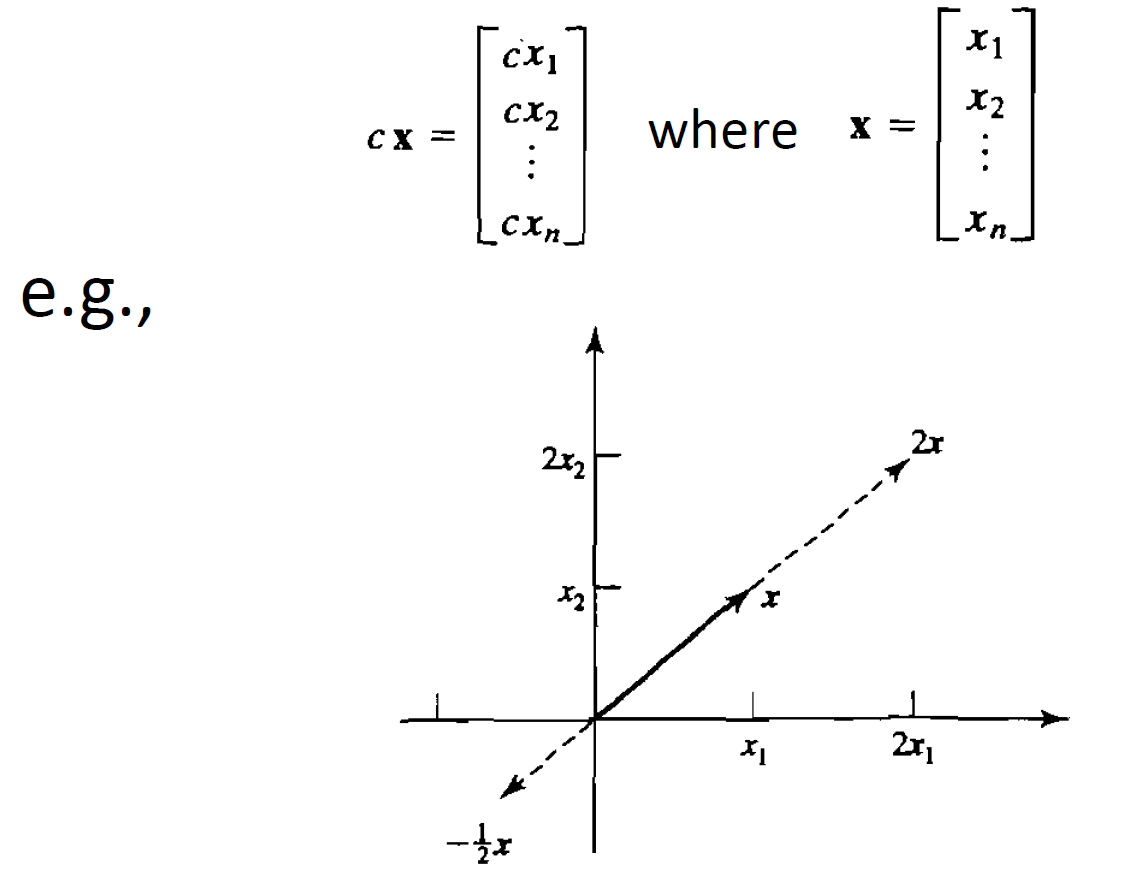
\includegraphics[width=0.6\linewidth]{img/VecScalarMultiplication}
\end{frame}

\begin{frame}[fragile]{Examples of Scalar Multiplication}
\protect\hypertarget{examples-of-scalar-multiplication}{}
\begin{Shaded}
\begin{Highlighting}[]
\NormalTok{x}\OtherTok{=}\FunctionTok{matrix}\NormalTok{(}\FunctionTok{c}\NormalTok{(}\FloatTok{0.4}\NormalTok{,}\FloatTok{0.2}\NormalTok{,}\FloatTok{0.5}\NormalTok{), }\DecValTok{3}\NormalTok{, }\DecValTok{1}\NormalTok{)}
\DecValTok{10}\SpecialCharTok{*}\NormalTok{x}
\end{Highlighting}
\end{Shaded}

\begin{verbatim}
##      [,1]
## [1,]    4
## [2,]    2
## [3,]    5
\end{verbatim}
\end{frame}

\begin{frame}{Addition and Substraction}
\protect\hypertarget{addition-and-substraction}{}
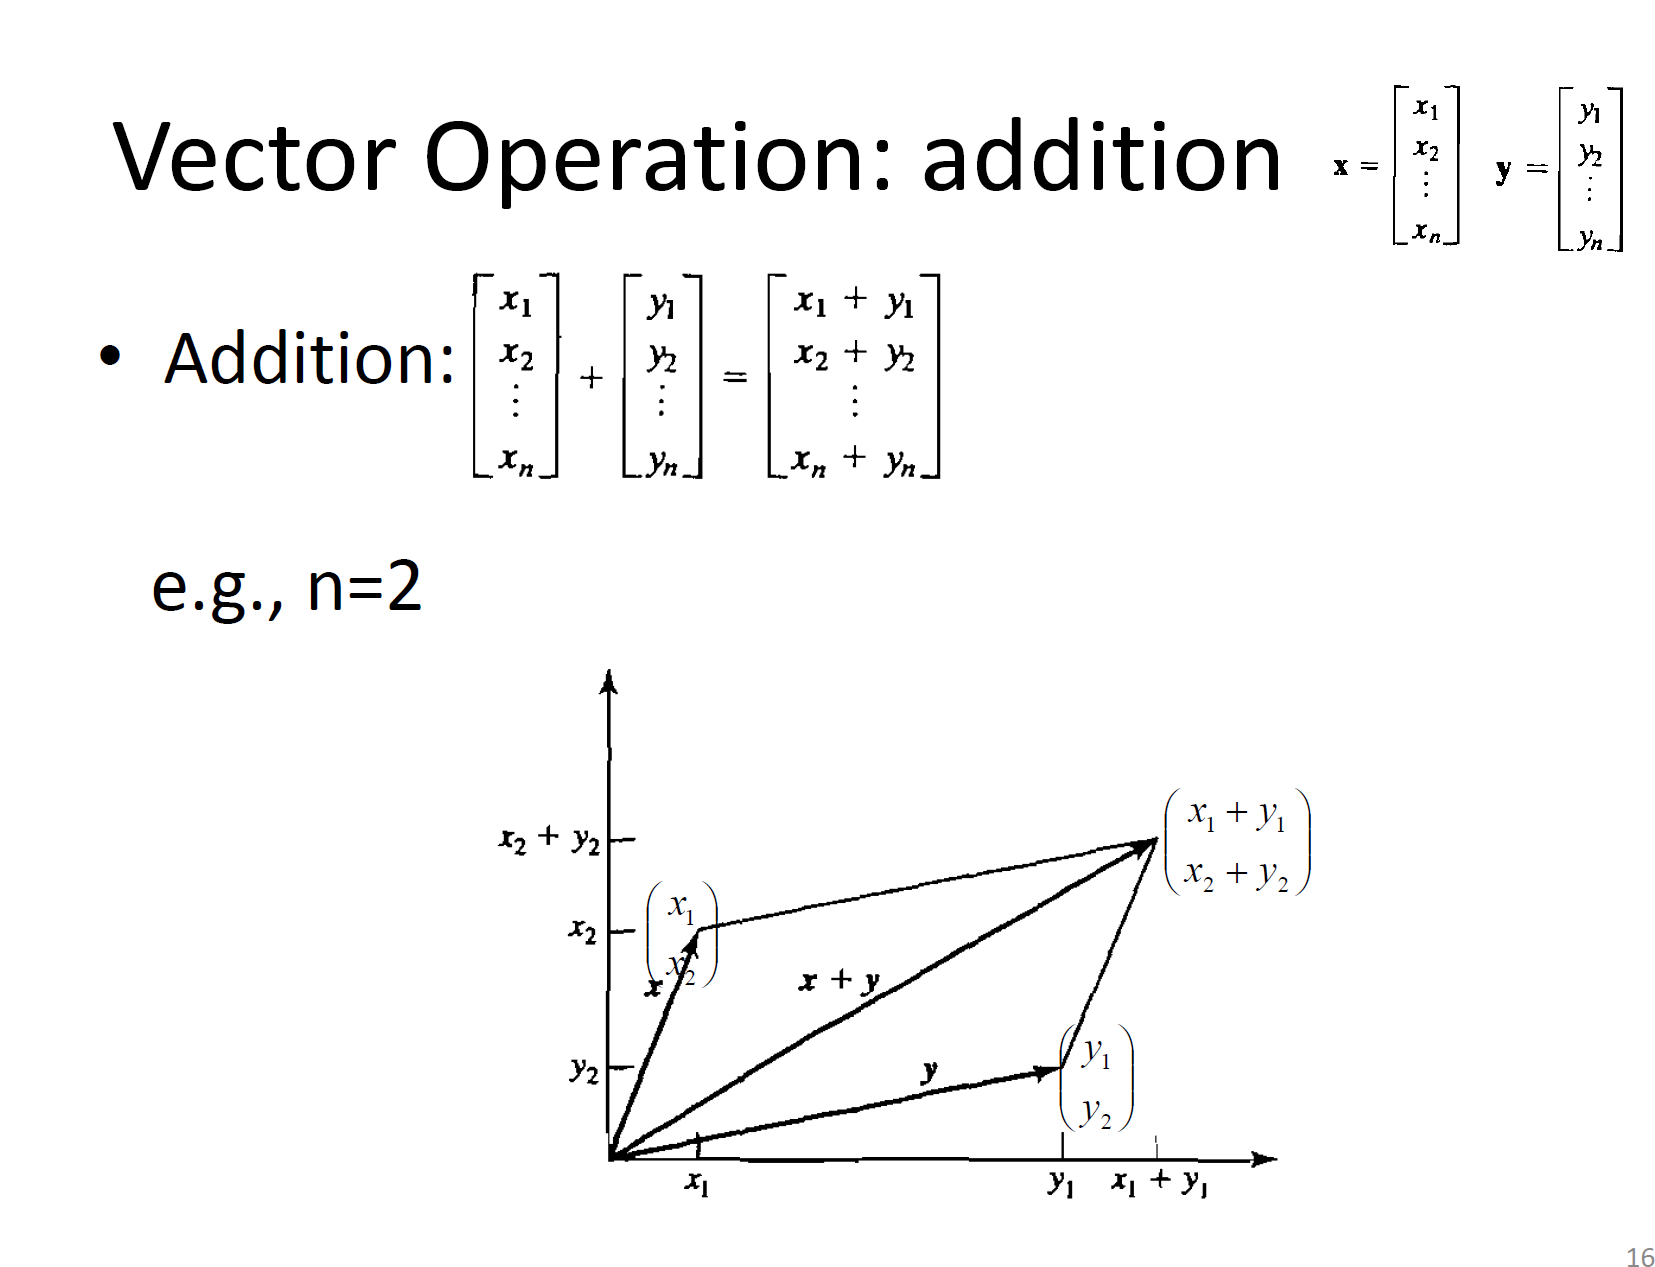
\includegraphics[width=0.7\linewidth]{img/VecAddition}
\end{frame}

\begin{frame}[fragile]{Example of Addition and Substraction}
\protect\hypertarget{example-of-addition-and-substraction}{}
\begin{Shaded}
\begin{Highlighting}[]
\NormalTok{x1}\OtherTok{=}\FunctionTok{matrix}\NormalTok{(}\FunctionTok{c}\NormalTok{(}\FloatTok{0.4}\NormalTok{,}\FloatTok{0.2}\NormalTok{,}\FloatTok{0.5}\NormalTok{), }\DecValTok{3}\NormalTok{, }\DecValTok{1}\NormalTok{)}
\NormalTok{x2}\OtherTok{=}\FunctionTok{rep}\NormalTok{(}\DecValTok{1}\NormalTok{, }\DecValTok{3}\NormalTok{)}
\NormalTok{x1}\SpecialCharTok{+}\NormalTok{x2}
\end{Highlighting}
\end{Shaded}

\begin{verbatim}
##      [,1]
## [1,]  1.4
## [2,]  1.2
## [3,]  1.5
\end{verbatim}

\begin{Shaded}
\begin{Highlighting}[]
\NormalTok{x1}\SpecialCharTok{{-}}\NormalTok{x2}
\end{Highlighting}
\end{Shaded}

\begin{verbatim}
##      [,1]
## [1,] -0.6
## [2,] -0.8
## [3,] -0.5
\end{verbatim}
\end{frame}

\begin{frame}{Outer Product}
\protect\hypertarget{outer-product}{}
\begin{itemize}
\tightlist
\item
  The outer product of two vectors \(x=(x_1,\cdots, x_m)'\) and
  \(y=(y_1,\cdots,y_n)'\) is \[x\otimes y= \begin{pmatrix}
  x_1y_1 & x_1y_2 & \cdots & x_1y_n\\
  \cdots& \cdots& \cdots& \cdots \\
  x_my_1 & x_my_2 & \cdots & x_my_n
  \end{pmatrix}\]
\item
  A similar operation for matrices is called Kronecker product.
\end{itemize}
\end{frame}

\begin{frame}[fragile]{Example: outer product}
\protect\hypertarget{example-outer-product}{}
\begin{Shaded}
\begin{Highlighting}[]
\NormalTok{x1}\OtherTok{=}\FunctionTok{matrix}\NormalTok{(}\FunctionTok{c}\NormalTok{(}\FloatTok{0.4}\NormalTok{,}\FloatTok{0.2}\NormalTok{,}\FloatTok{0.5}\NormalTok{), }\DecValTok{3}\NormalTok{, }\DecValTok{1}\NormalTok{)}
\NormalTok{x2}\OtherTok{=}\FunctionTok{rep}\NormalTok{(}\DecValTok{1}\NormalTok{, }\DecValTok{3}\NormalTok{)}
\NormalTok{x1}\SpecialCharTok{\%*\%}\NormalTok{x2}
\end{Highlighting}
\end{Shaded}

\begin{verbatim}
##      [,1] [,2] [,3]
## [1,]  0.4  0.4  0.4
## [2,]  0.2  0.2  0.2
## [3,]  0.5  0.5  0.5
\end{verbatim}
\end{frame}

\begin{frame}{Inner product}
\protect\hypertarget{inner-product}{}
\begin{itemize}
\tightlist
\item
  Let
  \(x=\begin{pmatrix}x_1\\ \cdots\\ x_n\end{pmatrix}, y=\begin{pmatrix}y_1\\ \cdots\\ y_n\end{pmatrix}\)
  The inner product of \(x\) and \(y\) is
  \[<x,y>=x_1y_1 + \cdots x_ky_n=\sum_{i=1}^n x_iy_i\]
\item
  Note, the two vectors must have the same length
\item
  The norm / Euclidean norm / length of \(x\) is \(||x||=\sqrt{<x,x>}\)
\item
  The Euclidean distance between \(x\) and \(y\) is
  \[D(x,y)=||x-y||=\sqrt{(x_1-y_1)^2 + \cdots (x_k-y_k)^2}\]
\end{itemize}
\end{frame}

\begin{frame}{Inner Product and Norm}
\protect\hypertarget{inner-product-and-norm}{}
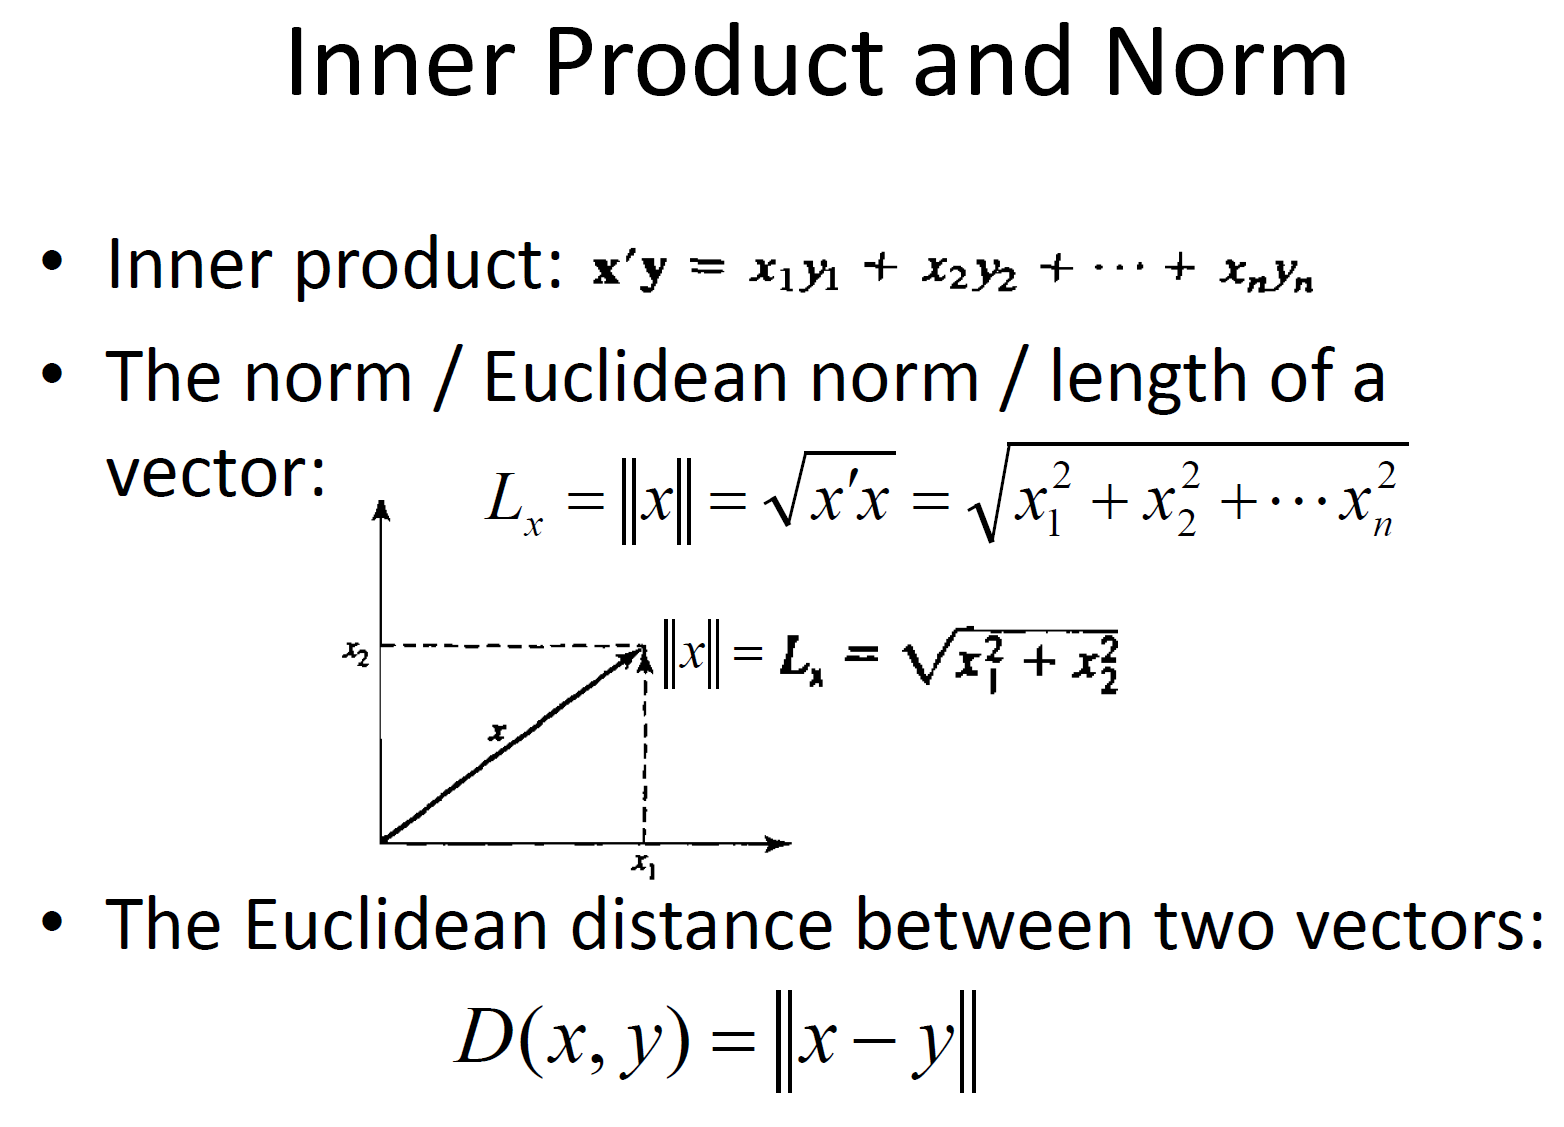
\includegraphics[width=0.7\linewidth]{img/InnerProdNorm}
\end{frame}

\begin{frame}{Distance: 1d and 2d}
\protect\hypertarget{distance-1d-and-2d}{}
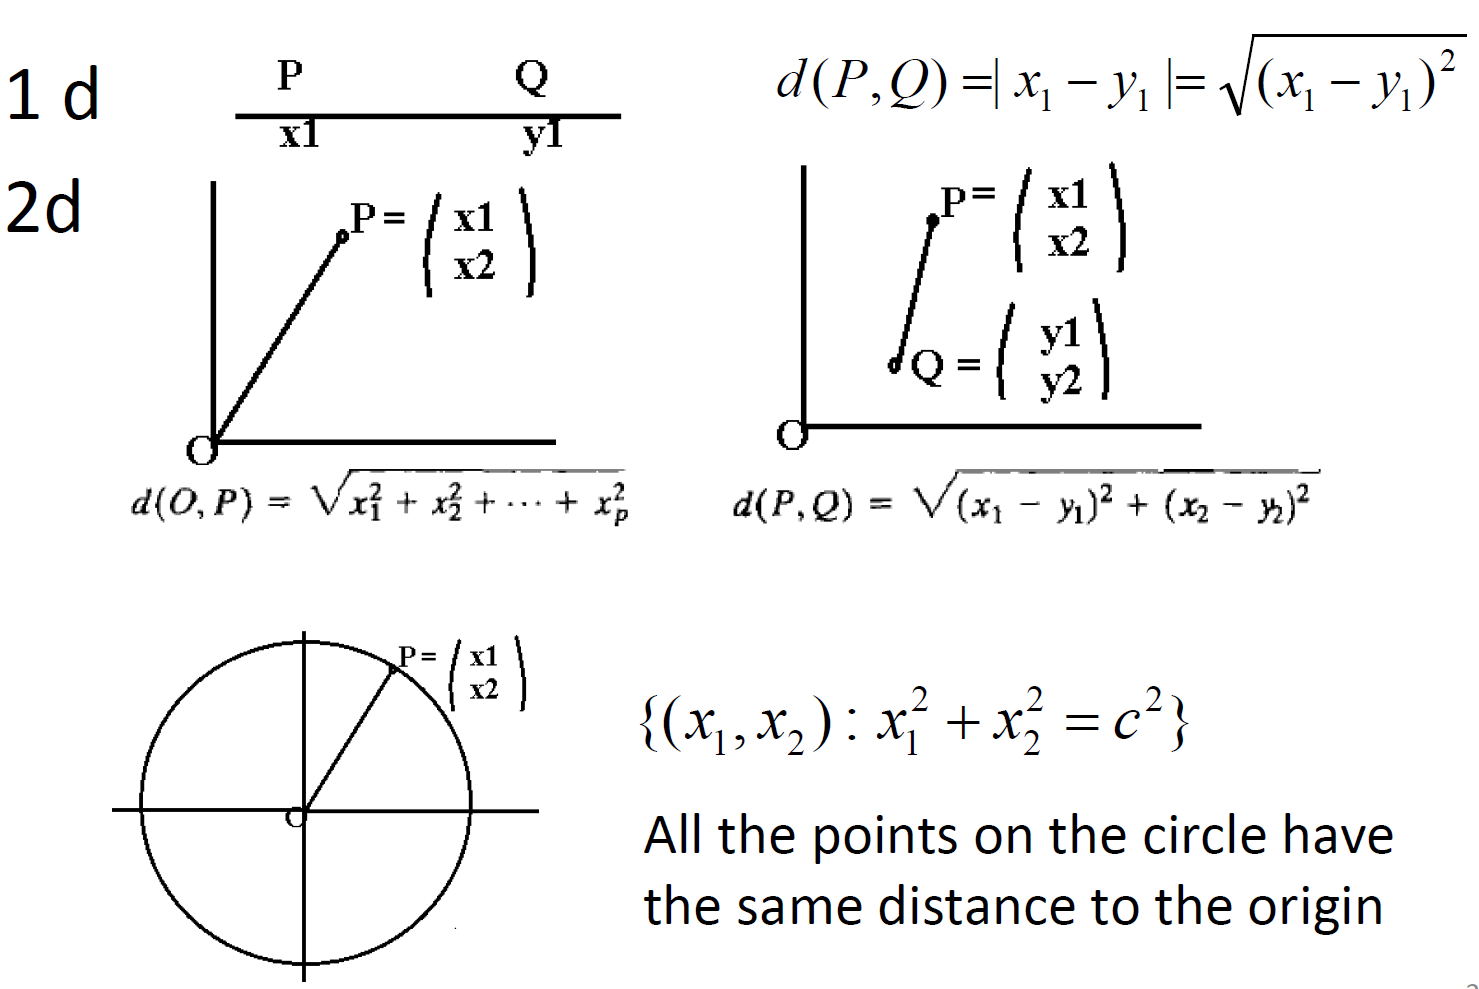
\includegraphics[width=0.7\linewidth]{img/Distance1d2d}
\end{frame}

\begin{frame}{Distance: 3d}
\protect\hypertarget{distance-3d}{}
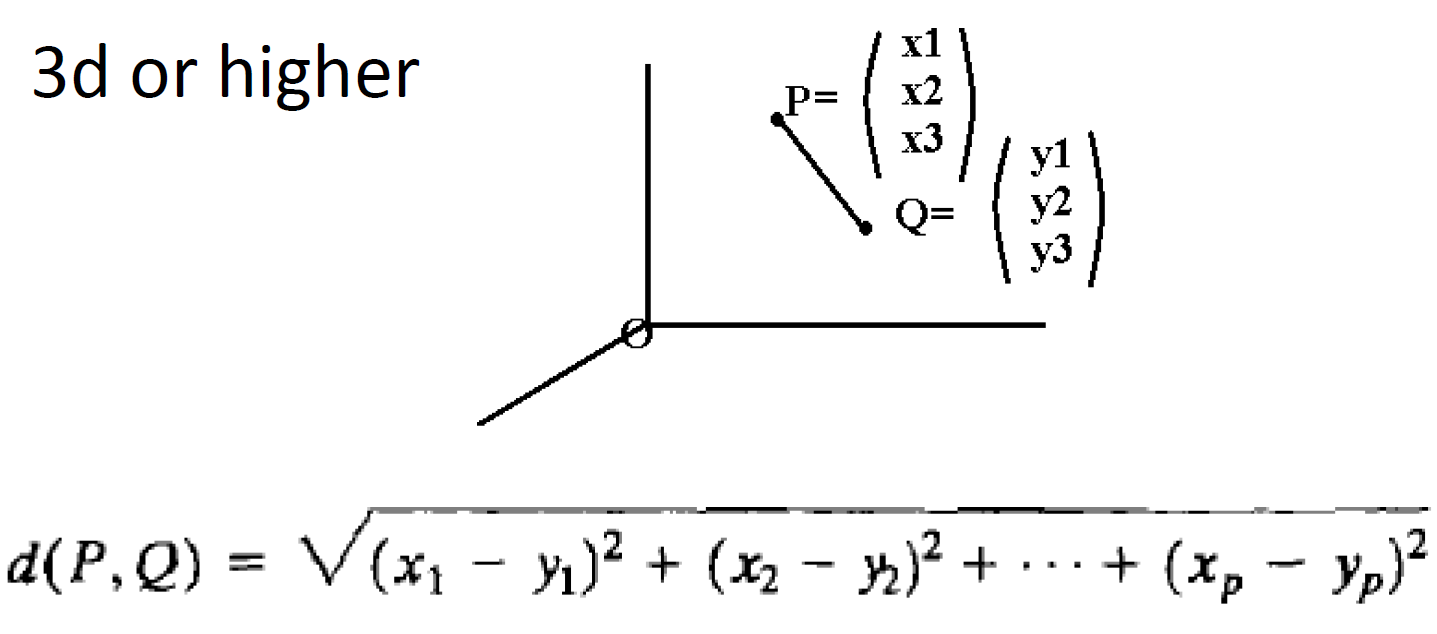
\includegraphics[width=0.8\linewidth]{img/Distance3d}
\end{frame}

\begin{frame}[fragile]{Example: Norm}
\protect\hypertarget{example-norm}{}
\begin{Shaded}
\begin{Highlighting}[]
\NormalTok{x1}\OtherTok{=}\FunctionTok{matrix}\NormalTok{(}\FunctionTok{c}\NormalTok{(}\FloatTok{0.4}\NormalTok{,}\FloatTok{0.2}\NormalTok{,}\FloatTok{0.5}\NormalTok{), }\DecValTok{3}\NormalTok{, }\DecValTok{1}\NormalTok{)}
\CommentTok{\#the norm/length of x1}
\FunctionTok{sqrt}\NormalTok{(}\FunctionTok{sum}\NormalTok{(x1}\SpecialCharTok{\^{}}\DecValTok{2}\NormalTok{))}
\end{Highlighting}
\end{Shaded}

\begin{verbatim}
## [1] 0.6708204
\end{verbatim}

\begin{Shaded}
\begin{Highlighting}[]
\CommentTok{\#or use pipe}
\NormalTok{x1}\SpecialCharTok{\^{}}\DecValTok{2} \SpecialCharTok{\%\textgreater{}\%}\NormalTok{ sum }\SpecialCharTok{\%\textgreater{}\%}\NormalTok{ sqrt}
\end{Highlighting}
\end{Shaded}

\begin{verbatim}
## [1] 0.6708204
\end{verbatim}
\end{frame}

\begin{frame}[fragile]{Example: (Euclidean) Distance}
\protect\hypertarget{example-euclidean-distance}{}
\begin{Shaded}
\begin{Highlighting}[]
\NormalTok{x1}\OtherTok{=}\FunctionTok{matrix}\NormalTok{(}\FunctionTok{c}\NormalTok{(}\FloatTok{0.4}\NormalTok{,}\FloatTok{0.2}\NormalTok{,}\FloatTok{0.5}\NormalTok{), }\DecValTok{3}\NormalTok{, }\DecValTok{1}\NormalTok{)}
\NormalTok{x2}\OtherTok{=}\FunctionTok{rep}\NormalTok{(}\DecValTok{1}\NormalTok{, }\DecValTok{3}\NormalTok{)}
\FunctionTok{sqrt}\NormalTok{(}\FunctionTok{sum}\NormalTok{((x1}\SpecialCharTok{{-}}\NormalTok{x2)}\SpecialCharTok{\^{}}\DecValTok{2}\NormalTok{))}
\end{Highlighting}
\end{Shaded}

\begin{verbatim}
## [1] 1.118034
\end{verbatim}

\begin{Shaded}
\begin{Highlighting}[]
\CommentTok{\#or use pipe}
\NormalTok{(x1}\SpecialCharTok{{-}}\NormalTok{x2)}\SpecialCharTok{\^{}}\DecValTok{2} \SpecialCharTok{\%\textgreater{}\%}\NormalTok{ sum }\SpecialCharTok{\%\textgreater{}\%}\NormalTok{ sqrt}
\end{Highlighting}
\end{Shaded}

\begin{verbatim}
## [1] 1.118034
\end{verbatim}
\end{frame}

\begin{frame}{Example: (Euclidean) Distance}
\protect\hypertarget{example-euclidean-distance-1}{}
\begin{itemize}
\tightlist
\item
  Motivating example. Consider bivariate random vectors. The standard
  deviations are 2 and 1, respectively.
\item
  What is the distance between (-2,0) and (2,0)? \textcolor{red}{4}.
\item
  What is the distance between (0, -2) and (0,2)? \textcolor{green}{4}.
\end{itemize}

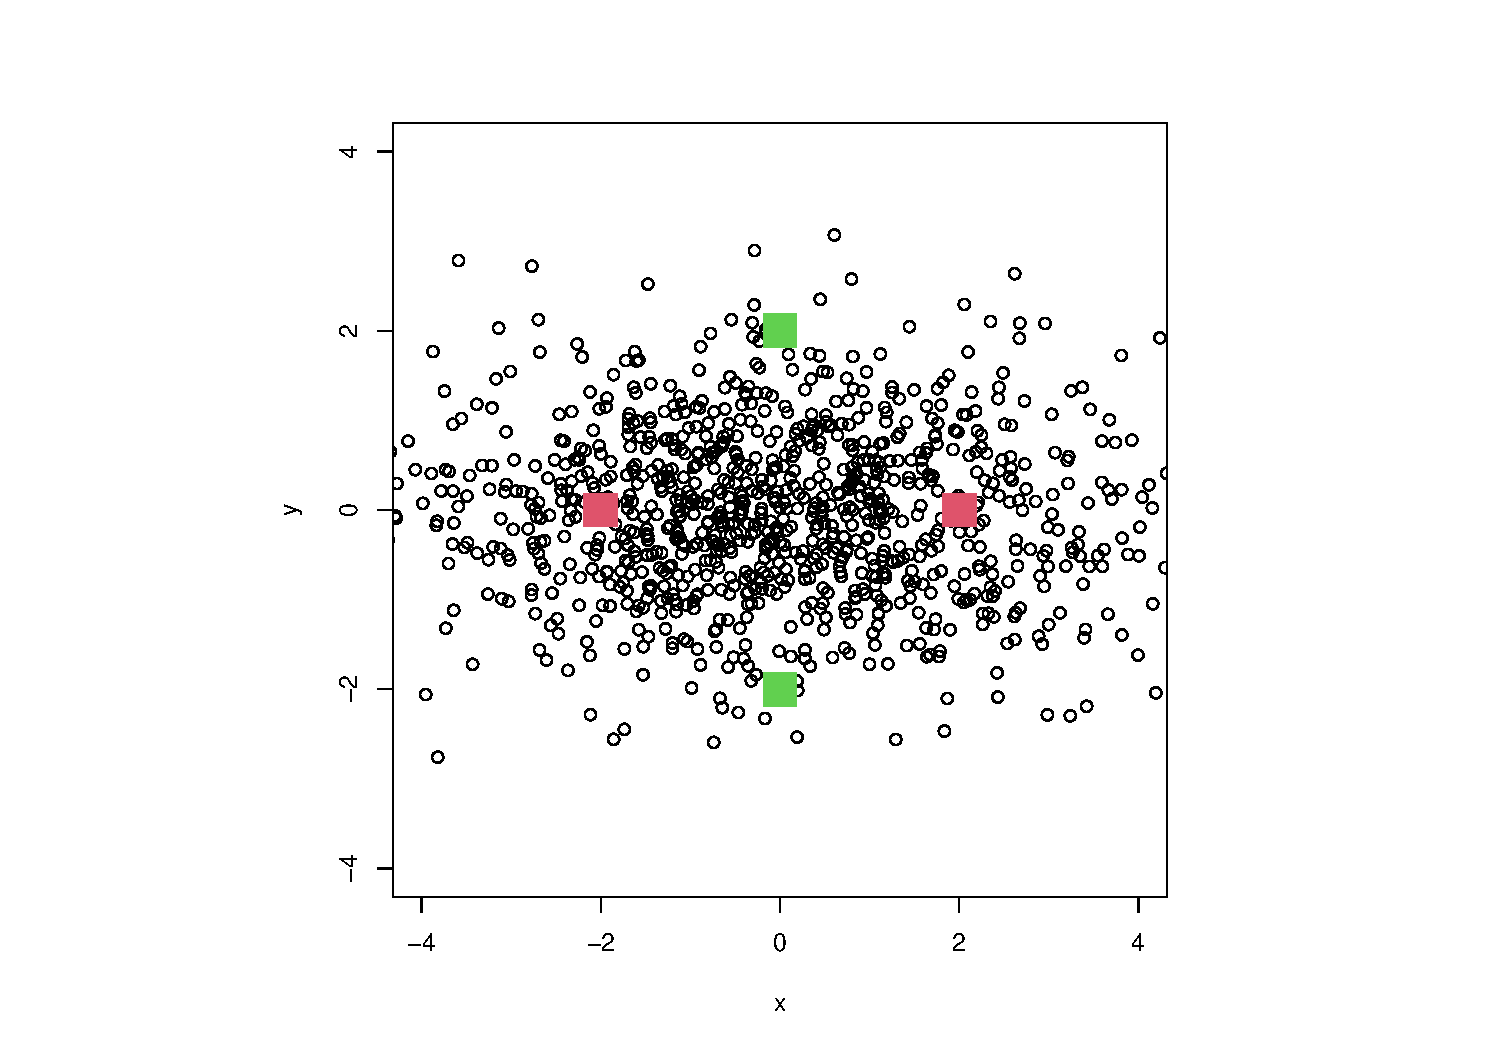
\includegraphics[width=0.6\linewidth]{Introduction_files/figure-beamer/unnamed-chunk-21-1}
\end{frame}

\begin{frame}[fragile]{Example: (Euclidean) Distance}
\protect\hypertarget{example-euclidean-distance-2}{}
\begin{Shaded}
\begin{Highlighting}[]
\CommentTok{\#R code}
\FunctionTok{set.seed}\NormalTok{(}\DecValTok{20230404}\NormalTok{)}
\FunctionTok{par}\NormalTok{(}\AttributeTok{pty=}\StringTok{"s"}\NormalTok{)}\CommentTok{\#to make sure the shape of figure is a square}
\FunctionTok{mvrnorm}\NormalTok{(}\AttributeTok{n=}\DecValTok{1000}\NormalTok{, }\FunctionTok{c}\NormalTok{(}\DecValTok{0}\NormalTok{,}\DecValTok{0}\NormalTok{), }\FunctionTok{matrix}\NormalTok{(}\FunctionTok{c}\NormalTok{(}\DecValTok{4}\NormalTok{,}\DecValTok{0}\NormalTok{,}\DecValTok{0}\NormalTok{,}\DecValTok{1}\NormalTok{),}\DecValTok{2}\NormalTok{,}\DecValTok{2}\NormalTok{)) }\SpecialCharTok{\%\textgreater{}\%} 
  \FunctionTok{plot}\NormalTok{(}\AttributeTok{xlab=}\StringTok{"x"}\NormalTok{, }\AttributeTok{ylab=}\StringTok{"y"}\NormalTok{, }\AttributeTok{xlim=}\FunctionTok{c}\NormalTok{(}\SpecialCharTok{{-}}\DecValTok{4}\NormalTok{,}\DecValTok{4}\NormalTok{), }\AttributeTok{ylim=}\FunctionTok{c}\NormalTok{(}\SpecialCharTok{{-}}\DecValTok{4}\NormalTok{,}\DecValTok{4}\NormalTok{))}
\FunctionTok{points}\NormalTok{(}\AttributeTok{x=}\FunctionTok{c}\NormalTok{(}\SpecialCharTok{{-}}\DecValTok{2}\NormalTok{, }\DecValTok{0}\NormalTok{, }\DecValTok{0}\NormalTok{, }\DecValTok{2}\NormalTok{), }\AttributeTok{y=}\FunctionTok{c}\NormalTok{(}\DecValTok{0}\NormalTok{, }\SpecialCharTok{{-}}\DecValTok{2}\NormalTok{, }\DecValTok{2}\NormalTok{, }\DecValTok{0}\NormalTok{), }\AttributeTok{pch=}\DecValTok{15}\NormalTok{, }
       \AttributeTok{col=}\FunctionTok{c}\NormalTok{(}\DecValTok{2}\NormalTok{,}\DecValTok{3}\NormalTok{,}\DecValTok{3}\NormalTok{,}\DecValTok{2}\NormalTok{),}\AttributeTok{cex=}\DecValTok{3}\NormalTok{)}
\end{Highlighting}
\end{Shaded}

\begin{itemize}
\tightlist
\item
  Both pairs have a distance of 4.
\item
  But we notice that the pairs with a y-distance greater than 4 is very
  rare; as a comparison, there are much pairs with a x-distance greater
  than 4.
\end{itemize}
\end{frame}

\begin{frame}{A Homework Problem of Euclidean Distances}
\protect\hypertarget{a-homework-problem-of-euclidean-distances}{}
\begin{itemize}
\tightlist
\item
  Suppose \(X_1, X_2, Y_1, Y_2\) are mutually independent.

  \begin{itemize}
  \tightlist
  \item
    \(X_1\) and \(X_2\) are iid from \(N(\mu=0, \sigma_x^2=2^2)\)
  \item
    \(Y_1\) and \(Y_2\) are iid from \(N(\mu=0, \sigma_y^2=1^2)\)
    Consider the two pairs \((X_1, X_2)\) and \((Y_1, Y_2)\). Which pair
    tends to have a larger difference? To answer the question, please
    calculate and estimate the following two probabilities:
    \[P(|X_1-X_2|>4), P(|Y_1-Y_2|>4)\]
  \end{itemize}
\item
  The hints for calculating/estimating \(P(|X_1-X_2|>4)\) can be found
  in the two slides. Using similar strategies, you can
  calculate/estimate \(P(|Y_1-Y_2|>4)\)
\end{itemize}
\end{frame}

\begin{frame}{Calculate \(P(|X_1-X_2|>4)\)}
\protect\hypertarget{calculate-px_1-x_24}{}
\begin{itemize}
\tightlist
\item
  Hints for calculating \(P(|X_1-X_2|>4)\).

  \begin{itemize}
  \tightlist
  \item
    First find the distribution of \(X_1-X_2\). Then standard it to have
    mean 0 and SD 1.
  \item
    Second, express the probability to \(P(|Z|>z)\), where
    \(Z\sim N(0,1)\).
  \item
    Next, expression the probability in terms of \(\Phi(\cdot)\), the
    CDF of the standard normal distribution.
  \item
    Last, use the ``pnorm'' function in R to find the numerical value.
  \end{itemize}
\end{itemize}
\end{frame}

\begin{frame}{Estimate \(P(|X_1-X_2|>4)\)}
\protect\hypertarget{estimate-px_1-x_24}{}
\begin{itemize}
\tightlist
\item
  The probability can be estimated by doing simulations/sampling.
\item
  If you sample many (say 10,000) pairs of \(X_1\) and \(X_2\), count
  how many pairs satisfying \(|X_1-X_2|>4\). The probability can be used
  to estimate \(P(|X_1-X_2|>4)\)
\end{itemize}
\end{frame}

\begin{frame}{Statistical / Mahalanobis Distance}
\protect\hypertarget{statistical-mahalanobis-distance}{}
\begin{itemize}
\tightlist
\item
  The two probabilities are quite different, suggesting that the
  Euclidean distance might be misleading given the joint distribution of
  the variable.
\item
  In this example we have examined, the x-values and y-values are
  independent. * The variation along \(x\) is greater than along \(y\).
  Let \(X_1\) and \(X_2\) be two random points along the \(x\)
  direction, \(Y_1\) and \(Y_2\) be two random points along the \(y\)
  direction.\\
\item
  One simple idea is to standardize both. Because the SD of Y is 1 we
  don't need to change the y-values. Because the SD of X is 2, we shrink
  the x-values by 50\%.

  \begin{itemize}
  \tightlist
  \item
    point (-2,0) becomes (-1,0)
  \item
    point (2, 0) becomes (1,0)
  \end{itemize}
\item
  The distance between the red pair is 2, the distance between the green
  pair is 4.
\end{itemize}
\end{frame}

\begin{frame}{Standardized Observations}
\protect\hypertarget{standardized-observations}{}
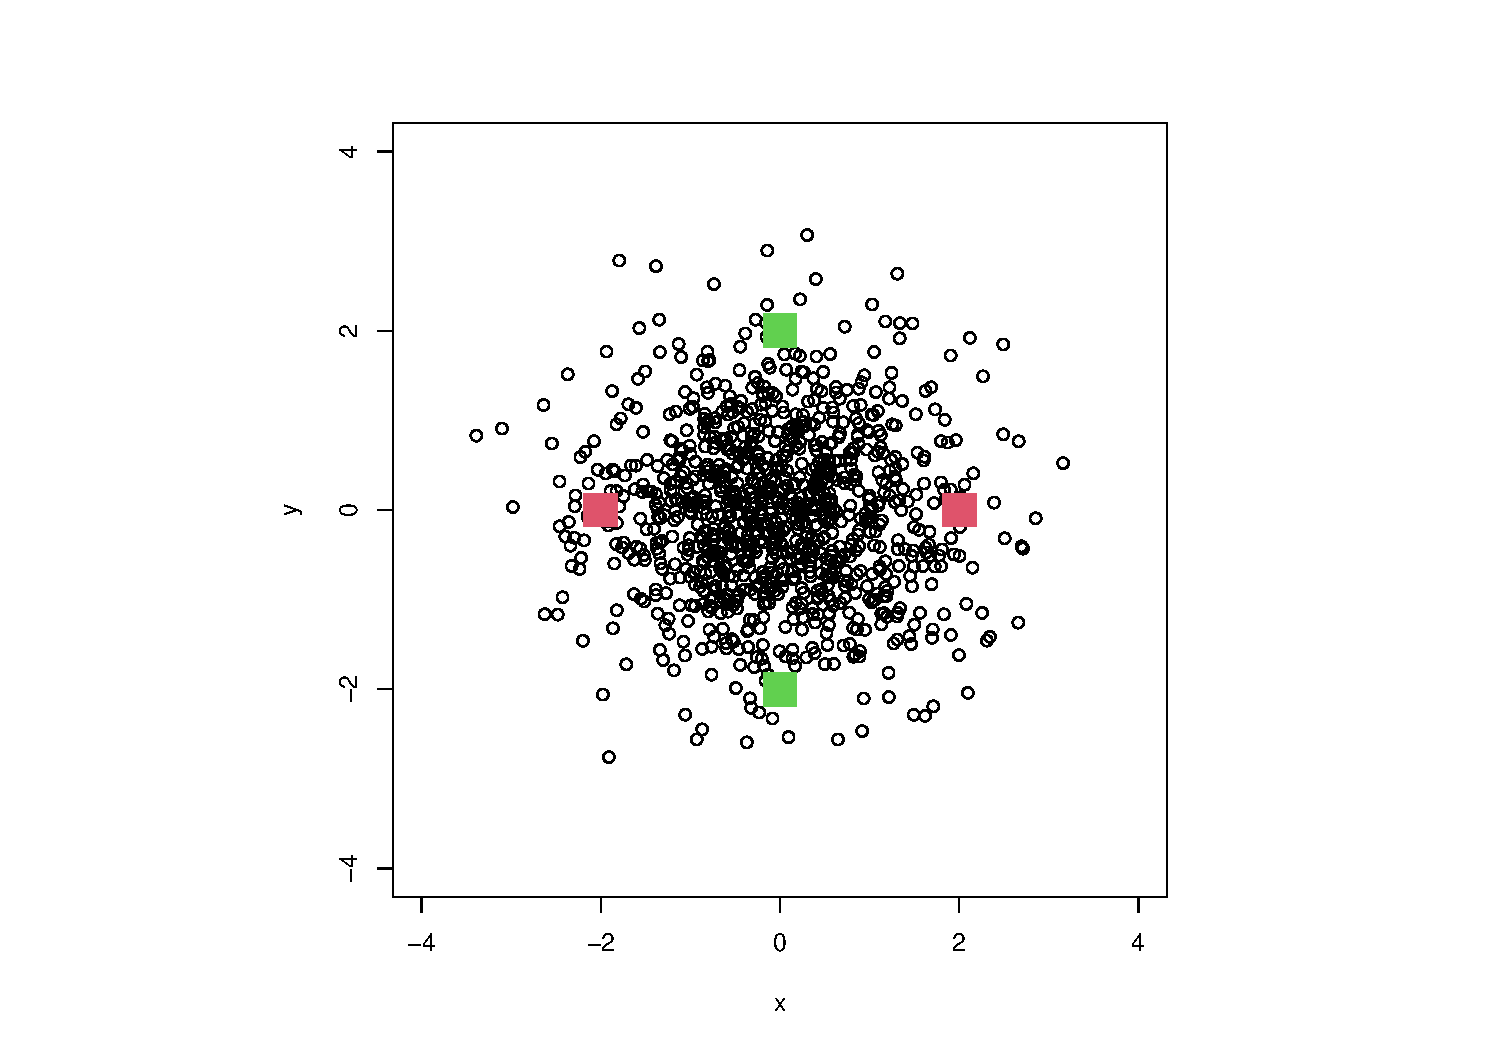
\includegraphics[width=0.6\linewidth]{Introduction_files/figure-beamer/unnamed-chunk-23-1}
\end{frame}

\begin{frame}{Standardized Observations}
\protect\hypertarget{standardized-observations-1}{}
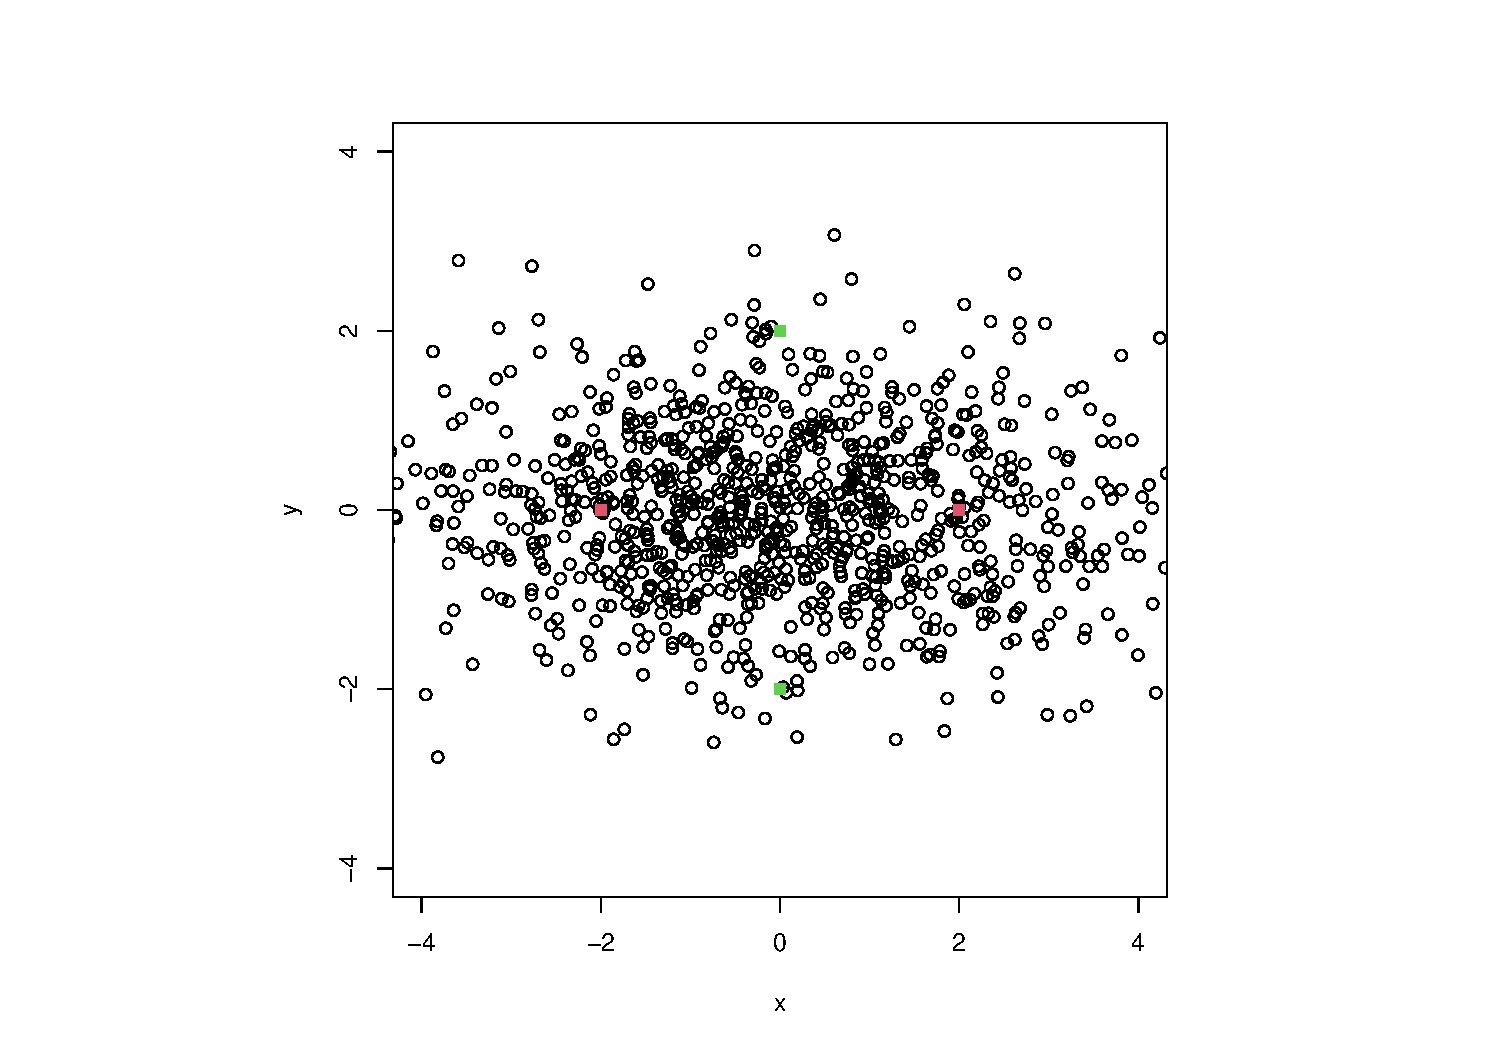
\includegraphics[width=0.6\linewidth]{Introduction_files/figure-beamer/unnamed-chunk-24-1}
\end{frame}

\begin{frame}{Statistical Distance}
\protect\hypertarget{statistical-distance}{}
\begin{itemize}
\tightlist
\item
  In The example above \(X\) and \(Y\) are independent, as a result, the
  covariance is zero. Statistical distance can also be defined when the
  covriance matrix \(\Sigma\) is not diagonal;
\item
  We will introduce a type of statistical distance, which is known as
  Mahalanobis distance.
\end{itemize}

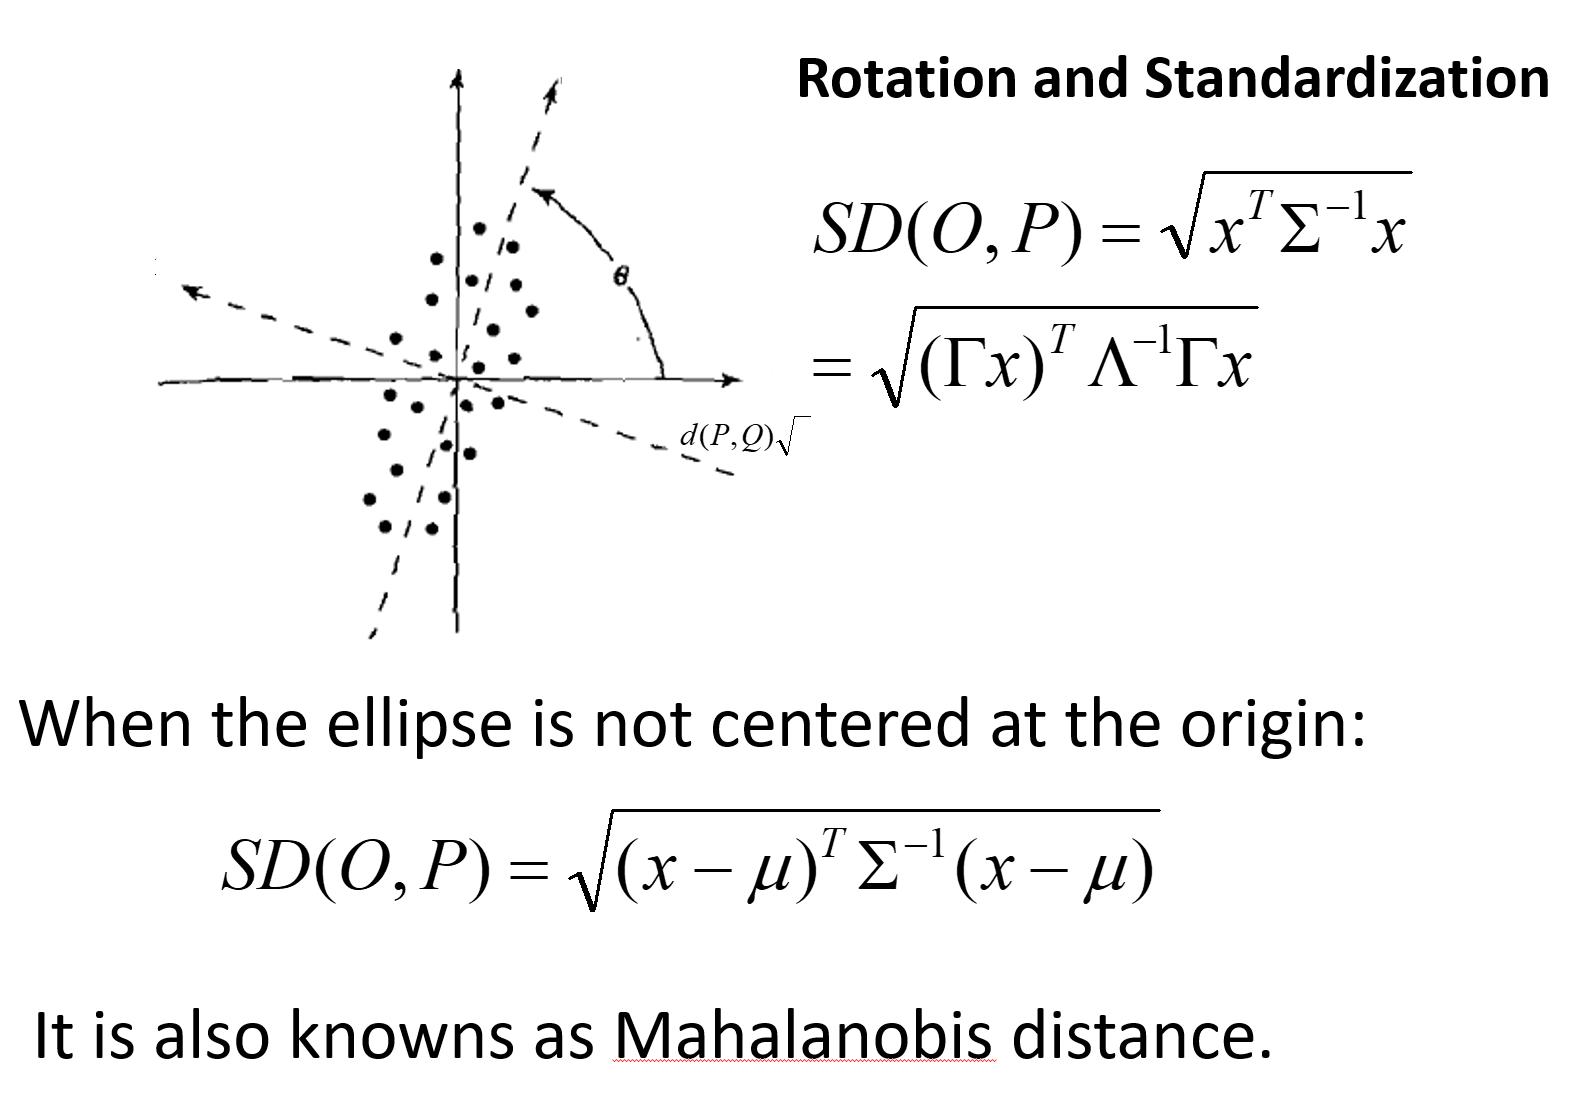
\includegraphics[width=0.6\linewidth]{img/StatDistance}

--\textgreater{}
\end{frame}

\end{document}
